\section{Current system}\label{sec:currsys}

At the moment, there are no mobile solutions to the already existing XOmail system on computers.

\subsection{XOmail - Secure message based information handling}

XOmail is a message system tailored for messaging within military organizations. The messaging functions within the system are suited for the needs of large organizations with the ability to differentiate between social messages to the entire organization and personal messages to individual users. XOmail has the ability to send messages to predefined  distribution lists where the messages gets distributed based on a given criteria like the subject of the message. 
\cite{bib:XOhome}
\newline
\newline
The system also has several APIs that can be accessed by other applications. XOmail supports message coordination for use in the drafting process, as well as the ability to have a release authority for a drafted message. Another feature of XOmail is the ability to add precedence to messages, giving high priority messages access to resources and communication channels before messages with lower precedence. This is very important in a military setting. 
\cite{bib:XOhome}
\newline
\newline
XOmail has also a high focus on security, and offers security for the messaging platform, servers and gateways. The system also has an extensive administration tool that can be accessed both locally and remotely.
\cite{bib:XOhome}
\newline
\newline

\begin{figure}[h!]
\begin{center}
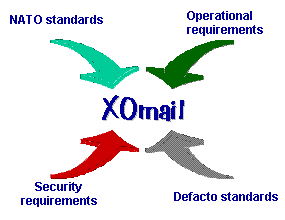
\includegraphics{xomaillogo}
\end{center}
\caption{XOmail logo} \label{fig:xomail}
\end{figure}